\section{Reproducibility Summary}

\subsection*{Scope of Reproducibility}

StylEx is an approach for classifier-conditioned training of a StyleGAN2 model \cite{karras2020analyzing}, intending to capture classifier-specific attributes in its disentangled StyleSpace \cite{9577297}. Attributes can be adjusted to generate counterfactual explanations of the classifier decisions. StylEx is domain and classifier-agnostic, while its explanations are claimed to be human-interpretable, distinct, coherent and sufficient to produce flipped classifier decisions. We verify these claims by reproducing a selection of the experiments in the paper.


\subsection*{Methodology}

We verified a selection of the experimental results on the code available by the authors. However, the training procedure, network architecture and hyperparameter configurations were missing. As such, we re-implemented the model and available TensorFlow code in PyTorch, to enable a more comprehensive reproducibility of the proposed case studies. All experiments were run in approximately 20-50 GPU hours per dataset, depending on the batch size, gradient accumulation and GPU used.


\subsection*{Results}

We verified that the publicly available pre-trained model has a 'sufficiency' measure within 1\% of the value reported in the paper. Additionally, we evaluate the \textit{Fréchet inception distance} (FID) scores of images generated by the released model. We show that the FID score increases with the number of attributes used to generate a counterfactual explanation. Custom models were trained on three datasets, with a reduced image dimensionality ($64^2$px). Additionally, a user study was conducted to evaluate the distinctiveness and coherence of the images. We report a significantly lower accuracy in the identification of the extracted attributes and 'sufficiency' scores on our model.


\subsection*{What was easy}

It was easy to run the provided Jupyter Notebook, and verify the results of the pre-trained models on the FFHQ dataset. Extending an existing StyleGAN2 model implementation to fit this study was relatively easy.


\subsection*{What was difficult}

Reproducing the experiments on the same scale as the authors, as well as the development of the full training procedure, model architecture and hyperparameters, particularly due to underspecification in the original paper. Additionally, the conversion of code from TensorFlow to PyTorch.


\subsection*{Communication with original authors}

We corresponded with the first author of the paper through several emails. Through our mail contact, additional details were released on the network architecture, the training procedure and the hyperparameter configurations.

\clearpage

\begin{figure}[!htb]
\minipage{0.32\textwidth}
  \includegraphics[width=\linewidth]{../openreview/Images/OldFaces/attribute_1.png}
\endminipage\hfill
\minipage{0.32\textwidth}
  \includegraphics[width=\linewidth]{../openreview/Images/Plants/attribute_1.png}
\endminipage\hfill
\minipage{0.32\textwidth}
  \includegraphics[width=\linewidth]{../openreview/Images/NewFaces/attribute_1.png}
\endminipage\hfill
\caption{Top-1 automatically detected attributes for perceived-gender classifiers (left: version 1, right: version 2) and perceived-health of leaves classifiers (middle). Similarly to the original paper, the counterfactual images are marked by a frame. Displayed probabilities correspond to the person being male for `perceived gender' and the leaf being healthy for `perceived health'. More attributes can be found in the appendix.}
\end{figure}


\section{Introduction}

\begin{comment}
In recent years, many machine learning algorithms have been designed to be black-box algorithms -- systems where everything is known about the inputs and the outputs, but little about the internal logic to the user. The lack of explanation introduces both a practical and an ethical issue and has hindered the large-scale deployment of these models \cite{guidotti2018survey}. 
\end{comment}

Existing post hoc visual explainability measures, such as heatmaps\cite{8237336}, can highlight regions that influence model decisions. However, they do not visualize non-spatially localized attributes, nor do they indicate how these areas may be changed to influence the classification. Counterfactual explanations, which are statements of the form "Had the input $\mathbf{x}$ been $\mathbf{x^{\prime}}$, the classifier output would have been $\mathbf{y^{\prime}}$ instead of $\mathbf{y}$", has been proposed as an alternative which both allows for the visualization of salient features and directly explains how they can be altered to achieve an alternative classification. 

As such, these explanations are promising as they can provide a suggestive recourse to non-domain experts in a machine learning-based decision system. The effectiveness of visual methods strongly depends on the intuitive difference that humans observe; therefore one of the primary objectives is to find interpretable, salient attributes. Secondary objectives involve the visualization and control of the impact of these attributes on the classifier output. 

In this work, we reproduce the paper ‘Explaining in Style: Explaining a GAN in StyleSpace’ \cite{explaining_in_style}. The paper proposes a novel method for explaining the classification of a given image, by altering discovered human-interpretable features discovered to affect the classification output. We re-implemented the model in PyTorch together with the unreleased training procedure, as the original TensorFlow implementation lacked the training procedure code. We performed training on the FFHQ and PlantVillage dataset using a lower resolution. Using our implementation, we check whether the results are consistent with the descriptions provided in the paper. We substantiate this with the addition of a human-grounded evaluation of the generated images. Additionally, we used the FID measure to evaluate the image quality of the counterfactual generated images.


\section{Scope of Reproducibility}

The StylEx model, in addition to the \textit{AttFind} algorithm defined in the paper, is presented as a viable option for generating counterfactual explanations of black-box classifiers. The StylEx procedure aims to make individual style coordinates classifier-relevant, through a novel training procedure which is outlined in \ref{methodology}. As no benchmark metrics exist to evaluate and assess attribute-based counterfactual explanations, the authors propose three evaluation criteria themselves: 1) visual coherence, 2) distinctness and 3) `effect of attributes on classification' (sufficiency). We reformulate these criteria as the main claims of the paper in the following manner: 

\begin{enumerate}
    \item \label{claim1}\textbf{Visual Coherence:} Attributes detected by StylEx should be clearly identifiable by humans.
    \item \label{claim2}\textbf{Distinctness:} The attributes extracted by StylEx should be distinct.
    \item \label{claim3}\textbf{Sufficiency:} Changing attributes should result in a change of classifier output, where changing multiple attributes has a cumulative effect.
\end{enumerate}

\section{Methodology}
\label{methodology}

To evaluate claim \ref{claim1} and \ref{claim2}, the authors conduct a user study in two parts. To evaluate claim \ref{claim3}, they study the percentage of flipped classifications when modifying top-$k$ (in their case $k=10$) attributes. To reproduce these claims, we conduct the same experiments, albeit at a lower dimensionality of $64^2$px. The complex network architecture of StyleGAN, as well as the encoder, requires a significant number of training epochs until its convergence and thus, training these at the full resolution of $256^2$px is extremely computationally expensive.

We verify the sufficiency scores of the released model, by making use of the supplied Jupyter Notebook. However, several elements crucial for reproduction were missing, including the training procedure, the omission of hyperparameter configurations and the details on the optimization procedure. As such, we ported the available TensorFlow code to PyTorch, and implemented the missing parts, to enable a more comprehensive reproducibility of StylEx.

We reimplemented the StylEx procedure in PyTorch, using an open-source StyleGAN2 model implementation as a starting point\footnote{https://github.com/lucidrains/stylegan2-pytorch}.

For running our code, we have made use of an NVIDIA GTX 1080 Ti, RTX 2070 Super and a laptop RTX 3060 graphics card, running on different machines. In the conduction of the user study, we have made use of the online survey tool Qualtrics \cite{qualtrics}.


\begin{comment}
The \href{https://github.com/google/explaining-in-style}{Jupyter Notebook} made available with the paper loads a pre-trained StylEx model, which is used to find and visualize classifier-specific attributes on the FFHQ dataset. The paper itself provided very little information on the implementation details of the StylEx framework. An open-source implementation in TensorFlow 2.7 was provided by the original authors, in the form of a Jupyter Notebook. However, it was quickly noted that this notebook lacked crucial elements to reproduce this research:

\begin{itemize}
    \item The only model that was provided was a StylEx model (or rather a multitude of models that encompass a singular StylEx model), which was fully trained on the FFHQ dataset with a perceived age classifier. The other datasets and classifiers reported were missing.
    \item The training code, including the hyperparameter configurations, was entirely missing from the notebook. While we could not obtain access to the training procedure code, through contact with the primary author the specifics of the optimization procedure were clarified, including the used hyperparameters configurations.
\end{itemize}

For these reasons, we have opted for a PyTorch implementation of the StylEx model and corresponding training procedure. Due to computational limitations, we evaluate the trained models on a subset of datasets present in the paper, with a reduced dimensionality of the generated images. 


The notebook does contain a TensorFlow implementation of their \textit{AttFind} algorithm, which we translated into PyTorch code for our implementation.
\end{comment}


\begin{figure}[h!]
    \centering
    \includegraphics[scale=0.4]{../openreview/Images/final-2.png}
    \caption{\textbf{StylEx network architecture:} with the respective classifier $C$, generator $G$, discriminator $D$ and encoder $E$. For clarification, we have slightly adapted the visualization to include the StyleVectorizer which obtains the latent vector $w$ from $z$ \cite{karras2019style}, after learning that the authors have used alternating training \ref{alternate training}}
    \label{fig:network-architecture}
\end{figure}

\subsection{Model descriptions}

In addition to a pre-trained classifier $C$, StylEx is comprised of three trainable elements, which are a 1) generator $G$,  2) a discriminator $D$ and 3) an encoder $E$. The $D$ and $G$ follow the StyleGAN2 model architecture, with minor alterations to $D$ which will be explained below. Figure \ref{fig:network-architecture} provides an overview of the network architecture.

Some design details were unspecified or omitted in the original paper. We contacted the authors to provide clarification on these details, which are stated as follows:
\begin{enumerate}
    \item StylEx is trained using both encoder input and noise input transformed through StyleGAN2's mapping network, using alternating steps; \label{alternate training}
    \item The output of $D$ is a weighted sum of the 2-dimensional output of its last layer with the classifier probabilities of the 1) original image if using the encoder, 2) randomly sampled image if using noise input; \label{point:discriminator_point}
    \item $\mathcal{L}_{rec}$ and $\mathcal{L}_{cls}$ are only calculated during the generator training steps.
\end{enumerate}

The GAN is trained jointly with the encoder, which embeds an image into the $W$ latent space of StyleGAN2, forming a latent vector $w$. A recent observation by \cite{wu2020stylespace} highlighted the disentanglement of this space (called StyleSpace) that is used in StylEx to extract classifier-specific attributes. Logits of the original image $C(x)$ are then appended to $w$, to condition the training on classifier inputs. The current architecture includes a StyleVectorizer that obtains the latent vector $w$ from $z$, which is sampled from a normal distribution. In alternating steps, the generator was fed input from the encoder and input from the StyleVectorizer mapping network \cite{karras2019style}. The original authors noticed a slight improvement in image quality using alternating training, compared to only using the encoder input.

Note that we used two slightly different implementation choices for training our models. The first implementation does not include the discriminator change mentioned in \ref{point:discriminator_point}, while the second implementation does and uses probabilities instead of logits for concatenation to $w$. We call these two choices `Model 1' and `Model 2' in results on datasets where we have trained both. We additionally noted that the MobileNet classifier `Model 1' was trained with did not perform well on the faces. This is why, for both faces models, a ResNet classifier was used to perform the AttFind algorithm. Additionally, we skipped discriminator filtering for `Model 2'. Discriminator filtering skips encoded images the discriminator deems unrealistic. We did this because the discriminator was too unstable to give reliable estimates. This might explain the poor performance of this model. We are unsure if this was caused by the changes to the architecture, training time or just bad luck.

This expanded latent vector $w$, either obtained by the encoder or StyleVectorizer, is passed on to the StyleGAN2 model, where it is transformed into the StyleSpace by a set of concurrent affine transformations to style vectors $s_{0}, ..., s_{n}$. These style vectors are used to generate novel images, that aim to reconstruct the original image as closely as possible. Several losses are used to aid the training procedure. The cumulative training loss for the algorithm is a sum of losses, denoted as follows:

\begin{equation}
\textrm{StylEx}_\textrm{Loss} = \mathcal{L}_{adv} + \mathcal{L}_{reg} + \mathcal{L}_{rec} + \mathcal{L}_{cls}.    
\end{equation}

A logistic adversarial loss \cite{goodfellow2014generative} $\mathcal{L}_{adv}$ is used as in standard GAN training, followed by the regularization loss $\mathcal{L}_{reg}$, as described in the original StyleGAN \cite{karras2020analyzing} paper. The reconstruction loss $\mathcal{L}_{rec}$ is given by the sum of  $\mathcal{L}_{rec}^x + \mathcal{L}_{rec}^w + \mathcal{L}_{LPIPS} $, where the first two terms are the $\mathbf{L1}$ distance between original and reconstructed input image, and the original and reconstructed $w$ latent vector, respectively. The $\mathcal{L}_{LPIPS}$ term is the LPIPS distance between original and reconstructed input, as described in \cite{8578166}. This loss ensures that reconstructed images resemble the original input as close as possible, to serve as an input for generating counterfactual examples. The classifier loss is defined as the Kullback-Leibler divergence between the original input image $X$ and the newly generated image $G(E(X), C(X))$ , defined as follows: $\mathcal{L}_{cls} = D_{KL}[|C(x')||C(x)]$. This loss ensures that the generator does not disregard image attributes that are important for the classification. 

To extract classifier-specific attributes, the \textit{AttFind} algorithm is proposed in the paper. As input, it takes the trained model $\mathcal{D}$ and a set of $N$ images of which the predicted labels do not match the target label $y$. For each class label, \textit{AttFind} encodes the images and iteratively tries to find a set $S_{y}$ of $M$ style coordinates that represent the largest possible shift to the opposing class. Next to this, it finds the set of directions $D_{y} \in \{\pm1\}^M$ in which the attribute needs to be adjusted to flip the classifier decision. In each iteration, it considers all style coordinates $K$ and determines the coordinate with the largest effect. All images in which changing this coordinate results in a large effect on their probability are removed from the iteration. The process is repeated until no images are left, or until $M$ attributes are found.


\subsection{Datasets}

We reproduce a selection of the findings of the authors on two of the given datasets in our PyTorch implementation:

\begin{enumerate}
    \item \textbf{CelebA \cite{liu2015faceattributes}}  The original Large-scale CelebFaces Attributes (CelebA) dataset\footnote{https://www.kaggle.com/jessicali9530/celeba-dataset} contains 200000 image entries, each containing 40 attribute annotations. We have trained classifiers on the `perceived gender' attribute.
    \item \textbf{FFHQ  \cite{orel2020lifespan}} The original Flickr-Faces-HQ dataset containing 70000 images of human faces. This dataset was used for StylEx training, while the pre-trained classifier was trained on the CelebA dataset, following the procedure of the original paper.\footnote{This is a detail that was revealed through contact with the authors.} 
    \item \textbf{Plant-Village:} This dataset contains 54303 entries of plant images, with 38 categories. This dataset was used to train the classifier to differentiate between sick and healthy leaves.
\end{enumerate}


For the classification tasks, the FFHQ dataset was split into train/validation/test sets of $70/15/15$, while the Plant-Village retained a proportion of $70/20/10$.

\subsection{Hyperparameters}

\textbf{Original research:} For the partial reproduction of Table 3 of the original paper, we limited ourselves to a sample of $n=250$ images, rather than the $n=1000$ randomly sampled images, as denoted in the \href{https://github.com/google/explaining-in-style}{Jupyter Notebook}.

\textbf{Reimplementation:} The computational costs of training StylEx precluded an in-depth hyperparameter search. For all modules except the encoder, we found a learning rate of $2e-4$ for the Adam optimizer, with $\beta_1 = 0.5$ and $\beta_2 = 0.9$. We found the training to diverge unless the encoder learning rate was lowered significantly to  $1e-5$. We ascribe this difference to the significantly smaller input size in our models or subtle implementation differences from the original paper that are unknown to us.

The classifier used in the paper was MobileNetV1 \cite{howard2017mobilenets}, but we opted for a MobileNetV2 \cite{sandler2019mobilenetv2} or ResNet-18 models\cite{7780459}. The authors asserted that the use of advanced networks identified more subtle cues from the datasets on the classification problems at hand, and for this purpose, we opted for ResNet-18. Additionally, we observed that the MobileNet model did not perform well on the CelebA dataset for gender classification on this image resolution. The components of the $\mathcal{L}_{rec}$ loss were scaled according to authors' suggestion in our correspondence: $0.1$ for $\mathcal{L}_{rec}^x$ and $\mathcal{L}_{LPIPS}$, 1 for $ \mathcal{L}_{rec}^w$. Other loss components were not scaled.

On the local GPUs, we used a batch size of 4 with 8 gradient accumulation steps, while we use a batch size of $16$ with $4$ gradient accumulation steps on the computer cluster. For the training of the MobileNet V2 classifier and the ResNet-18 classifier, we finetuned the pretrained models by slowly unfreezing the top layers, we have set the learning rate to $lr = 1e-4$, used a batch size of 128 and used the Adam \cite{kingma2017adam} with default PyTorch parameters.
 

\subsection{Experimental setup and code}

We aimed to follow the experimental setup as close as possible for our experiments. Our PyTorch implementation is available on GitHub\footnote{https://github.com/NoahVl/Explaining-In-Style-Reproducibility-Study} to further support and advance reproducibility in machine learning research. The repository provides explanations to run the described experiments.


\subsection{Computational requirements} 

Locally, our models were trained on two different machines, which contained a 1) laptop NVIDIA RTX 3060, 2) an NVIDIA RTX 2070 Super. A computer cluster containing GTX 1080 Ti GPUs was also used to train some of our models. The first machine makes use of the Windows operating system, while the latter two are Linux-based. For both the FFHQ dataset as well as the Plant-Village dataset, training was done until convergence, which was reached in 150K training steps for the FFHQ dataset and 260K training steps on the Plant-Village dataset. 

On the local GPUs, a batch size of 4 (RTX 3060) and 8 (RTX 2070 Super) was used alongside gradient accumulation for 8 (RTX 3060) and 2 (RTX 2070 Super) steps. On the computer cluster, a batch size of 16 was used, with a gradient accumulation parameter of 4. Depending on the hyperparameters of the batch size and gradient accumulation, the computational time to run the experiments ranged between 20-50 GPU hours. Training for 150000 steps took 20 hours on an RTX 2070 Super.


\section{Results}
\label{sec:results}


\subsection{Results reproducing original paper}

\subsubsection{Sufficiency}

We calculate the percentage of flipped classifications after changing the top-$10$ most influential attributes found by the \textit{AttFind} procedure. The results can be seen in table \ref{tab:sufficiency}. Our results using the author's model are within 1\% of the accuracy reported in the paper. Our models show significantly worse performance on both perceived gender (51\% vs 83.2\%) and plant healthiness (30\% vs 91.2\%), showing that the attributes discovered are not very relevant for classification.

% \begin{table}[h]
%     \centering
%     \begin{tabular}{ c | c{2cm} }
%     \toprule
%     \textbf{Dataset} & \textbf{Ours} \\
%     \midrule
%     \textit{FFHQ - Perceived Age} & 94.8\% \\
%     FFHQ - Perceived Gender (Model 1, $s=2$) & 51\% \\
%     FFHQ - Perceived Gender (Model 2, $s=1$) & 21\% \\
%     Plant Village - Perceived Health ($s=2$) & 30\% \\
%     \bottomrule
%     \end{tabular}
%     \caption{Percentage of flipped classifications on different datasets. Row in $italics$ shows our experiment on the original authors' model. $s$ represents the shift size used to generate the results. The shift sizes have been chosen by qualitatively looking at the produced images.}
%     \label{tab:sufficiency}
% \end{table}

\begin{table}[h]
    \centering
    \begin{tabular}{ c | c }
    \toprule
    \textbf{Dataset} & \textbf{Ours} \\
    \midrule
    \textit{FFHQ - Perceived Age} & 94.8\% \\
    FFHQ - Perceived Gender (Model 1, $s=2$) & 51\% \\
    FFHQ - Perceived Gender (Model 2, $s=1$) & 21\% \\
    Plant Village - Perceived Health ($s=2$) & 30\% \\
    \bottomrule
    \end{tabular}
    \caption{Percentage of flipped classifications on different datasets. Row in $italics$ shows our experiment on the original authors' model. $s$ represents the shift size used to generate the results. The shift sizes have been chosen by qualitatively looking at the produced images.}
    \label{tab:sufficiency}
\end{table}


\subsubsection{Coherency and Distinctness}
Similar to the original paper, we have conducted a user study ($n=54$) to evaluate the distinctiveness of the found attributes and the coherence of the generated images. The user study was divided into two parts - 1) a classification study and 2) a verbal description study, following a similar setup as presented in \cite{yeh2020completenessaware}. For the classification study, users are shown one animation of four images in a grid format. The two images on the left switch between their original image and have the same transformation applied. The two images on the right swap between their original image and one of two transformations. The user then has to find the transformation on the right that matches with those on the left. In the verbal description study, the users were asked to look at an animation of four images, and consequently describe in 1-4 words the changing attribute.

We have done this for the plant dataset as well as the FFHQ datasets. The order of the datasets was randomized to avoid biases and learning effects. All participants are undergraduate and graduate students who have some affinity with and knowledge of machine learning. None of them reported having color blindness. In Appendix \ref{appendix:user-study}, a few examples can be found on the posed questions (without animations) and the type of provided answers. The full user evaluation data and questions from the questionnaire can be found on our GitHub repository, under the folder \texttt{all\_user\_studies}.

% \begin{table}[h!]
%     \centering
%     \begin{tabular}{ c | c{2cm} | c{2cm} | c{2cm} }
%     \toprule
%     \textbf{Dataset} & \textbf{Wu \emph{et al.}} & \textbf{Lang \emph{et al.}} & \textbf{Ours} \\
%     \midrule
%     FFHQ - Perceived Gender & 0.783 (±0.186) & 0.96 (±0.047) & \begin{tabular}[c]{@{}l@{}} Model 1: 0.52 (±0.2081)\\ Model 2: 0.79 (±0.1599)\end{tabular} \\
%     Plant Village - Perceived Health & 0.91 (±0.081) & 0.916 (±0.081) & 0.66 (±0.323) \\
%     \bottomrule
%     \end{tabular}
%     \caption{\textbf{User study results.} Partial reproduction of Table 2 of the original paper, on a subset of the datasets.}
% \end{table}

\begin{table}[h!]
    \centering
    \begin{tabular}{ c | c | c | c }
    \toprule
    \textbf{Dataset} & \textbf{Wu \emph{et al.}} & \textbf{Lang \emph{et al.}} & \textbf{Ours} \\
    \midrule
    FFHQ - Perceived Gender & 0.783 (±0.186) & 0.96 (±0.047) & \begin{tabular}[c]{@{}l@{}} Model 1: 0.52 (±0.2081)\\ Model 2: 0.79 (±0.1599)\end{tabular} \\
    Plant Village - Perceived Health & 0.91 (±0.081) & 0.916 (±0.081) & 0.66 (±0.323) \\
    \bottomrule
    \end{tabular}
    \caption{\textbf{User study results.} Partial reproduction of Table 2 of the original paper, on a subset of the datasets.}
\end{table}

Although our results seem to slightly outperform the results by Wu \emph{et al.} (2021) on the perceived gender classifier, it does not seem to outperform the method posed by Lang \emph{et al.} (2021).

\subsection{Results beyond original paper}

\subsubsection{FID scores}

\begin{wrapfigure}{hbt!}{0.37\textwidth}
\captionsetup{justification=centering}
    \resizebox{0.4\textwidth}{!}{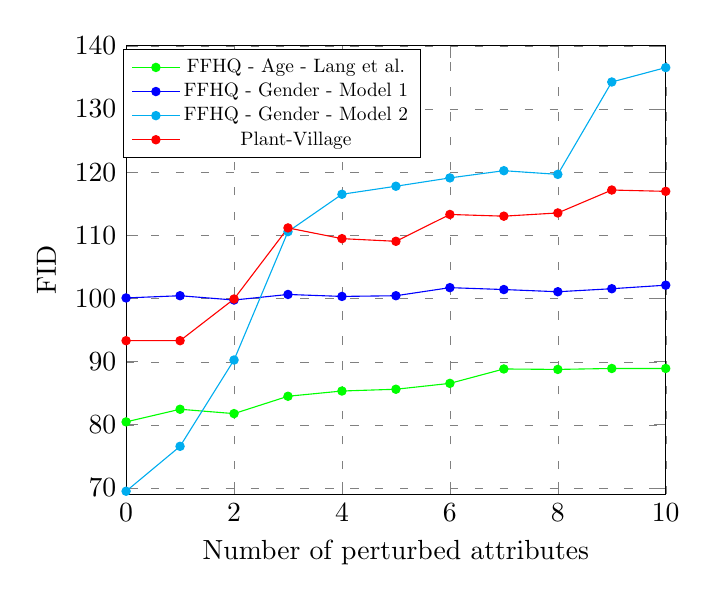
\begin{tikzpicture}
        \begin{axis}[anchor=north,
                     grid=both,
                     grid style={loosely dashed, gray, line width=.01pt},
                     xlabel = {Number of perturbed attributes},
                     ylabel = {FID},
                     xmin = 0,
                     xmax = 10,
                     ymin = 69,
                     ymax = 140,
                     xtick = {0, 2, 4, 6, 8, 10},
                     ytick={70, 80, 90, 100, 110, 120, 130, 140},
                     legend style={at={(0.27, 0.75)}, anchor=south, nodes={scale=0.7, transform shape}}, 
                     legend image post style={mark=*},
                     legend columns=1]
        \addlegendentry{FFHQ - Age - Lang et al.}
        \addplot[mark=*, thin, green, mark repeat=1, mark options={scale=0.75}] coordinates {
        (0, 80.44) (1, 82.44) (2, 81.75) (3, 84.50) (4, 85.33) (5, 85.61) (6, 86.54) (7, 88.82) (8, 88.75) (9, 88.90) (10, 88.90)};
        \addlegendentry{FFHQ - Gender - Model 1}
        \addplot[mark=*, thin, blue, mark repeat=1, mark options={scale=0.75}] coordinates {
        (0, 100.07) (1, 100.42) (2, 99.74) (3, 100.62) (4, 100.31) (5, 100.42) (6, 101.70) (7, 101.40) (8, 101.05) (9, 101.53) (10, 102.09)};
        \addlegendentry{FFHQ - Gender - Model 2}
        \addplot[mark=*, thin, cyan, mark repeat=1, mark options={scale=0.75}] coordinates {
        (0, 69.46) (1, 76.57) (2, 90.24) (3, 110.57) (4, 116.49) (5, 117.76) (6, 119.08) (7, 120.22) (8, 119.64) (9, 134.27) (10, 136.55)};
        \addlegendentry{Plant-Village}
        \addplot[mark=*,thin,red, mark repeat=1, mark options={scale=0.75}] coordinates {
        (0, 93.30) (1, 93.30) (2, 99.90) (3, 111.16) (4, 109.46) (5, 109.04) (6, 113.29) (7, 113.02) (8, 113.53) (9, 117.16) (10, 116.95)};
        \end{axis}
    \end{tikzpicture}}
    \caption{\label{fig:FID}FID scores after perturbing top-$k$ attributes.}
\end{wrapfigure}

To investigate the impact of attribute perturbation on the quality of the generated images, we compute the Fréchet Inception Distance (FID)  \cite{heusel2017gans} between the original images and the generated images, as described by \citet{Seitzer2020FID}. We perturbed the images with increasingly more attributes in a cumulative fashion, starting from zero perturbed attributes, which corresponds to only encoding and decoding the image. For the pre-trained model from the original authors, we used the provided subset of 250 latent vectors and their corresponding original images that were found in FFHQ. For our models, we used subsets of 100 images (500 images for model 2) due to computational constraints with regard to running the \textit{AttFind} algorithm. Our results, seen in \ref{fig:FID}, show that the FID increases with the number of stacked perturbed attributes.

This result is not surprising for three reasons. Firstly, making an image to be classified as another class might introduce perturbations for a certain class that are out-of-distribution for that particular class. For example, a man with lipstick does not appear often in the male class. Therefore, counterfactuals are more likely to be out of distribution to a particular degree. Secondly, a combination of perturbations seems to be more likely to produce an image that is more out of distribution than when one perturbation is applied individually. For example, a woman with thicker eyebrows in combination with more facial hair might be more out of distribution than one of those perturbations individually. Moreover, we noticed that perturbing several attributes leads to an increasing number of image artefacts, which could be an additional cause for the increasing FID score. This holds both for the original authors' models and our implementation.

\section{Discussion}

Our experimental results support the claims made in the original paper - the attributes detected by StylEx are identifiable by humans to a certain degree, distinct and sufficient. However, due to the significantly lower resolution and poorer image quality of the models, these results are not comparable to the ones displayed in the original paper.

\textbf{Reflection on our reproducibility study}
An important insight obtained during the conduction of the study is that the provided code did not cover the entire scope of the paper. Through a thorough study of both the code as well as the paper, we quickly noted discrepancies and missing elements that were fundamental - such as the network architecture, scaling of the losses and the hyperparameter configurations - to the original research. 
We believe that researchers could enhance transparency and reproducibility in machine learning research by the addition of a reproducibility statement within their research, including the used hardware, releasing written software and adding details relevant to the paper (e.g. such as clarifications on the exact network architecture). Moreover, it is important to detail hyperparameter search spaces and final parameter settings for all the used architectures and baselines. We believe that transparency is fundamental to stimulating the large-scale deployment of machine learning algorithms.

\subsection{What was easy}
It was relatively easy to run the code as the provided Jupyter Notebook by the authors. The provided notebook was thoroughly documented and written in a consistent coding style, making the interpretation of the notebook easier. However, the provided notebook lacked the elements to fully reproduce the research; the training procedure of the network was missing, only one pre-trained model was provided and four datasets were missing that we were required to add. As such, we had to implement the framework in PyTorch, while porting the limited released code from TensorFlow. Adding a dataset not used in the original notebook to accommodate the experiments was a relatively easy task.

\subsection{What was difficult}

Given the limited computational resources that were available to us, reproducing the experiments at the same computational scale as the authors were deemed to be the largest challenge. For the training of the model, the original authors made use of 8 NVIDIA V100s, which took the original authors a week to train at the full resolution of $256^2$px, whereas we were restricted to the use of the computer cluster, Colab/Kaggle, and our local GPUs. Due to this limitation, we had to scale down the resolution of the new images across the different datasets significantly. We scaled down the resolution of the generated images across the different datasets to a resolution of $64^2$px, which reduced the fidelity of the reconstructed images.  Additionally, we experienced the following issues with the original paper:

\begin{enumerate}
    \item \textbf{Little to no hyperparameters were given in the paper}, e.g. on the scaling of the losses, the learning rates etc;
    \item \textbf{Ambiguities about the training procedure}: the classifier in the notebook was trained on CelebA, instead of the FFHQ dataset, which we did not expect. This appeared to be a design choice by the authors, as the CelebA dataset contained labels, which the network could leverage information from. Additionally, softmax logits appeared to be added to the discriminator -- which was not mentioned explicitly in the paper -- but appeared to follow the cGAN \cite{mirza2014conditional} training procedure;
    \item \textbf{Ambiguities on the network architecture}: It was not entirely clear what the dimensionality and the function were of the $z$ vector, as the paper did not explicitly mention this;
    \item \textbf{Ambiguities about the preprocessing pipeline of the images} before it enters the encoder/classifier - in contact with the authors, they appeared to scale the RGB values from $[-1,1]$.
\end{enumerate}

The original authors did provide the hyperparameter configurations early on, which slightly reduced the time to explore the different possibilities, but the provided learning rate for example was too high for us. Additionally, the conversion of the \textit{AttFind} algorithm from TensorFlow to PyTorch also proved to be a somewhat difficult exercise. The challenge predominantly concerned the integration of this algorithm within the new PyTorch codebase, which required a thorough understanding of the internal workings of the algorithm.


\subsection{Communication with original authors}
Three emails were sent to the first author of the paper. In these emails, we have asked for additional details on the proposed network architecture, hyperparameter configurations and the training procedure of the networks. These details were not noted in the paper, nor in the provided code. Answers to these questions were provided promptly. Unfortunately, they were not able to share their code for the training procedure, as it contained too many internal dependencies from their perspective.
